\chapter{Implementación}
En el siguiente capítulo se describe la implementación del sistema desarrollado durante la memoria. Se implementaron dos posibles arquitecturas para un sistema de reconocimiento de videos. La primera alternativa graba videos con el dispositivo móvil y los envía completos al servidor, para que este calcule sus descriptores y realice la búsqueda, llamamos a esta la alternativa \emph{centralizada} pues todos los cálculos son realizados en el servidor. La segunda alternativa del sistema realiza los cálculos de descriptores en el mismo dispositivo móvil que graba el video, luego solo es necesario enviar los descriptores calculados al servidor que ejecuta la búsqueda, llamamos a esta alternativa \emph{distribuida} pues los cálculos están repartidos entre el cliente y el servidor.

En ambas versiones del sistema el cliente corresponde a una aplicación Android implementada en el lenguaje de programación Java, mientras que el servidor fue implementado en Python usando Flask\footnote{\url{http://flask.pocoo.org/}}, un framework minimal para programación de servicios web. Se decidió este ambiente de programación para el servidor dada la familiaridad del alumno memorista con el framework y porque la implementación del servidor no requiere funcionalidad compleja que justifique usar herramientas más completas.

El capítulo se divide en una sección para la alternativa centralizada y otra para la distribuida. A su vez cada sección se divide en la implementación del cliente Android y el servidor.


\section{Sistema Centralizado}

La figura~\ref{arquitectura_centralizada} muestra la arquitectura de la versión centralizada del sistema. En esta versión el dispositivo móvil es usado solo para grabar un video corto. El archivo de video resultante es enviado al servidor (1), el cual calcula sus descriptores (2) y realiza la búsqueda en la base de datos (3), devolviendo los resultados al cliente (4).
A continuación se detalla la implementación de esta versión del sistema, separando el cliente Android del servidor.
	\begin{figure}[!h]
		\centering
		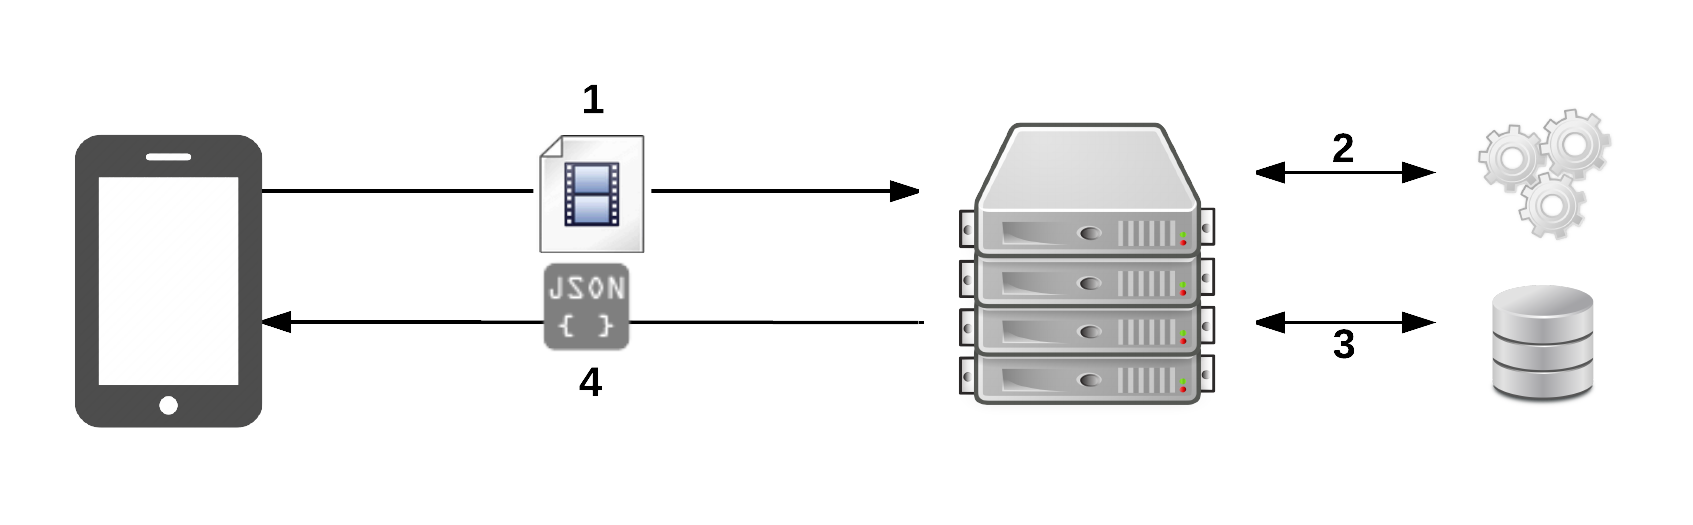
\includegraphics[scale=1]{imagenes/cap4/arquitectura_centralizada}
		\caption{Diagrama de la arquitectura del sistema centralizado.}
		\label{arquitectura_centralizada}
	\end{figure}
\subsection{Cliente Android}
En esta versión el cliente Android es responsable de grabar un video usando la cámara del dispositivo, enviarlo al servidor y de mostrarle al usuario los resultados de la búsqueda realizada por el servidor. Para cada una de estas responsabilidades se implementó un módulo.

\subsubsection*{Grabación}

El módulo de grabación es responsable de grabar un video usando la cámara del dispositivo y guardar el archivo resultante. Para lograr esto se creó el fragmento \texttt{VideoRecordFragment}, esta clase presenta al usuario un breve mensaje de instrucciones y un botón para comenzar la grabación. La figura ~\ref{pantalla_video_record_fragment} corresponde a la pantalla que ve el usuario al iniciar la aplicación. Al hacer click en el botón \emph{grabar} el sistema invoca a la aplicación por defecto de grabación de videos de Android por medio de un Intent.
La aplicación de grabación presenta un preview de la cámara como muestra la figura~\ref{pantalla_video_record_android}, en este momento el usuario debe iniciar la grabación, que dura por un máximo de 5 segundos y guarda en un archivo el video resultante. Después de terminar la grabación el sistema le cede de vuelta el control a la aplicación llamando al método \texttt{onActivityResult}, con esto se procede a enviar el video resultante al servidor.
\TODO{insertar aquí pantallazos de la aplicación}

\subsubsection*{Conexión con el servidor}
El módulo de conexión con el servidor es responsable de enviar al servidor el video capturado por el módulo anterior. Se implementó la clase \texttt{FromVideoSearchRequest} que recibe un archivo y ejecuta un petición HTTP Post al servidor usando la clase \texttt{HttpUrlConnection} de Java. Con la petición Post se envía el archivo grabado y un parámetro con el tipo de descriptor para usar en la búsqueda. Al crear un objeto de la clase \texttt{FromVideoSearchRequest} se le debe entregar un \texttt{ResponseHandler}, que corresponde a una interfaz con los métodos \texttt{onSuccessResponse} y \texttt{onFailure}, alguno de estos métodos se llamará dependiendo de la respuesta del servidor.
Una vez se termina el envío de datos al servidor se cambia la interfaz por una pantalla inicialmente vacía donde se mostraran los resultados como muestra la figura~\ref{pantalla_empty_results}.

\subsubsection*{Interfaz de resultados}
Para mostrarle los resultados de la búsqueda al usuario se implementó el fragmento \texttt{QueryResultsFragment} que implementa la interfaz \texttt{ResponseHandler} definida en la parte anterior. Inicialmente el fragmento muestra un texto indicando que se están esperando los resultados de la búsqueda, cuando se obtiene respuesta del servidor se ejecuta alguno de los métodos de la interfaz. Si el servidor responde con un error se ejecuta el método \texttt{onFailure} que muestra un mensaje al usuario informándolo del error. De lo contrario se ejecuta el método \texttt{onSuccessResponse} que recibe un String con los resultados del servidor codificados como JSON. Los resultados son deserializados usando la biblioteca GSON\footnote{GSON, biblioteca para convertir objetos Java a sus representación en JSON y vice-versa: \url{https://github.com/google/gson}} de manera que cada candidato de video identificado se convierte en un objeto de la clase \texttt{Detection} y se ingresa en una lista. El fragmento contiene un \texttt{ListView}, un elemento de interfaz de Android para mostrar listas de objetos. Se programó la clase \texttt{QueryResultAdapter} que recibe la lista de detecciones y crea una vista con cada una como muestra la figura~\ref{pantalla_list_results}.

El diagrama de la figura~\ref{diagrama_clases_centralizado} muestra las clases descritas en la sección anterior, detallando sus contenidos e interacciones.
	\begin{figure}[!h]
		\centering
		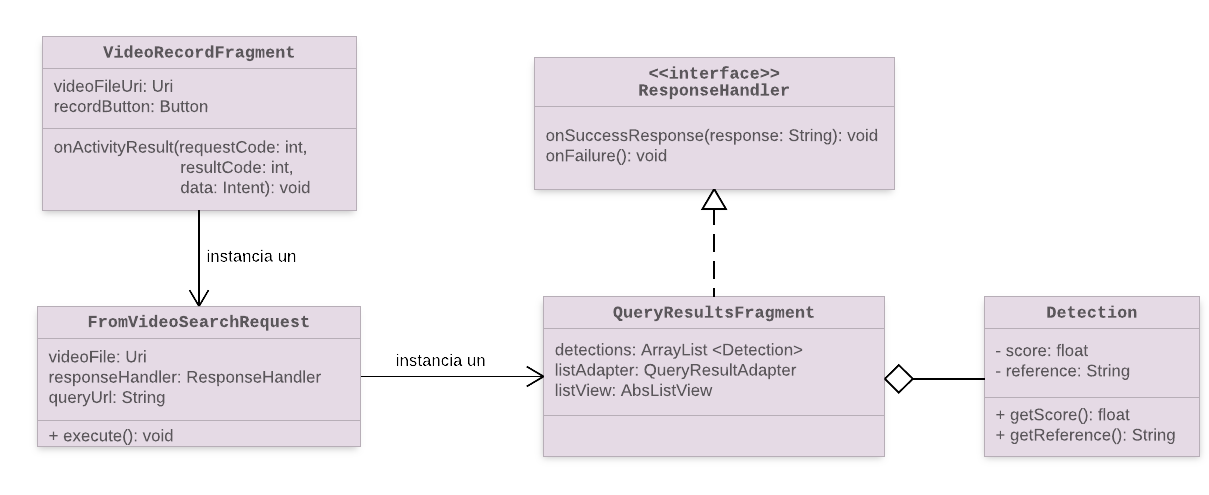
\includegraphics[scale=1.6]{imagenes/cap4/diagrama_cliente_centralizado.png}
		\caption{Diagrama de clases del cliente Android cetnralizado.}
		\label{diagrama_clases_centralizado}
	\end{figure}

\subsection{Servidor}

El servidor debe recibir una petición Post que contenga un video y el tipo de descriptor que se desea usar en la búsqueda. Debe usar el programa P-VCD para calcular los descriptores especificados y realizar la búsqueda para identificar el video original, finalmente debe entregarle al cliente en formato JSON una lista de los candidatos que encuentre.

Para recibir peticiones Post se usó el framework Flask, que permite programar servicios web con muy poco código extra. El siguiente ejemplo muestra todo el código necesario para definir y responder una petición Post:
\begin{lstlisting}[language=python]
from flask import Flask
app = Flask(__name__)

@app.route("/api/example/post", method=['POST'])
def hello():
	return "Hello World!"
	
if __name__ == "__main__":
	app.run(host='0.0.0.0')
\end{lstlisting}

La primera línea importa el módulo Flask, luego se define el objeto \texttt{app} que representa el contexto global de la aplicación. Para definir una request define una función con la anotación \texttt{@app.route}, explicitando la ruta y el tipo de petición. La función sirve una petición a la ruta especificada, dentro de la función se puede utilizar el objeto \texttt{app} para obtener el contenido de la petición. El string retornado por la función se convierte automáticamente en la respuesta del servidor.

Para servir la petición Post requerida se creó la función \texttt{search\_by\_video\_file} que escucha la URL host/api/search/search\_by\_video\_file.

\subsubsection*{Comunicación con P-VCD}
Como se detalló en capítulos anteriores P-VCD consta de múltiples módulos, cada uno con sus propio ejecutable que puede ser llamado por línea de comandos. Para usarlo en conjunto con el servidor para realizar el cálculo de descriptores y la búsqueda fue necesario encontrar la manera de ejecutar un programa externo desde Python.
Se encontró el módulo \texttt{subprocess}\footnote{Documentación del módulo subprocess: \url{https://docs.python.org/2/library/subprocess.html}} de Python que permite lanzar nuevos procesos pesados desde python de manera síncrona o asíncrona y obtener sus resultados. En particular se utilizó la función \texttt{call} de este módulo, que recibe una lista de strings con el nombre del programa y sus argumentos, lanza un nuevo proceso y espera a que termine, retornando el código de retorno del proceso.

Usando lo anterior se creó el módulo \texttt{PVCD\_Wrapper} que envuelve llamadas a las distintas etapas del proceso de búsqueda de P-VCD en funciones de python, a continuación se decriben las funciones usadas.
\begin{itemize}
\item \textbf{compute\_descriptors}: \\
La función recibe un archivo de video, un string correspondiente al tipo de descriptor a utilizar y un alias para el descriptor. Con esto realiza las llamadas necesarias para la extracción de descriptores de P-VCD, esto es, se llama a \texttt{pvcd\_db -new} para crear una nueva base de datos con el video correspondiente, luego se llama a \texttt{pvcd\_db -segment} para calcular su segmentación y finalemente se llama a \texttt{pvcd\_db -extract} para extraer el descriptor especificado.
\item \textbf{new\_search\_profile}: \\
Esta función recibe dos strings, uno con el nombre de la base de datos con los descriptores de consulta, y otro con el alias del descriptor y  realiza la llamada a \texttt{pvcd\_search -new} para crear un nuevo perfil de búsqueda.
\item \textbf{search}: \\
Esta función no recibe argumentos, llama a \texttt{pvcd\_search -ss} que toma los descriptores del video de consulta y para cada uno busca sus vecinos más cercanos en la base de datos de referencia.
\item \textbf{detect}: \\
Esta función no recibe argumentos llama a \texttt{pvcd\_detect} que usa la información de vecinos más cercanos del paso anterior para detectar secuencias al mismo video. P-VCD escribe en un archivo detections.txt la información de los videos que se consideran candidatos a ser el video original. La función lee este archivo y retorna una lista con el nombre de cada video y el puntaje de confianza que le asigna el sistema.

\end{itemize}
Usando estas funciones el código de la función \texttt{search\_by\_video\_file} queda como sigue:
\begin{lstlisting}[language=python]
@app.route("/search/api/search_by_video_file", methods=['POST'])
def search_by_video_file():
  if request.method == 'POST':
    uploaded_file = request.files['uploaded_file']
    if uploaded_file and allowed_file(uploaded_file.filename):
      db_name = 'query'
      descriptor = request.form['descriptor']
      alias = request.form['alias']
      file_path = save_video_file(uploaded_file)
      PVCD_Wrapper.compute_descriptors(file_path, descriptor, alias)
      PVCD_Wrapper.new_search_profile(db_name, alias)
      PVCD_Wrapper.search()
      detections = PVCD_Wrapper.detect()
      
      return jsonify(detections=detections)
\end{lstlisting}
Primero se verifica que la petición sea de tipo Post y que se haya recibido un video con formato válido. Luego la función ejecuta secuencialmente los pasos de la búsqueda y retorna los resultados usando la función \texttt{jsonify} de Flask, que codifica una lista de Python como JSON.


Esta versión del sistema destaca por su simplicidad y facilidad de implementar. Además el sistema resultante es flexible, puesto que tiene a su disposición todos los descriptores disponibles en P-VCD y solo se requieren cambios de configuración del servidor para cambiar el descriptor usado por el sistema. Sin embargo esta arquitectura presenta dos grandes problemas, por un lado enviar el video completo al servidor significa un considerable gasto de la red de datos del dispositivo. Por otro lado, el realizar todas las operaciones en el servidor se crea un posible cuello de botella que limita la escalabilidad del sistema. Ambos problemas se originan por el uso ineficiente de los recursos computacionales del sistema. No se está aprovechando la capacidad de computo del dispositivo móvil, en la siguiente sección se propone una arquitectura alternativa que busca solucionar estos problemas.


\section{Sistema Distribuido}

La figura~\ref{arquitectura_distribuida} ilustra la arquitectura de esta versión del sistema. El cálculo de descriptores para la búsqueda es realizado por el cliente Android (1) utilizando las herramientas para computación paralela descritas en secciones anteriores. Una vez calculados, se envían solo estos descriptores al servidor (2) el cual los usa para realizar la búsqueda por similitud (3) y luego comunica los resultados de vuelta al cliente (4).

	\begin{figure}[!h]
		\centering
		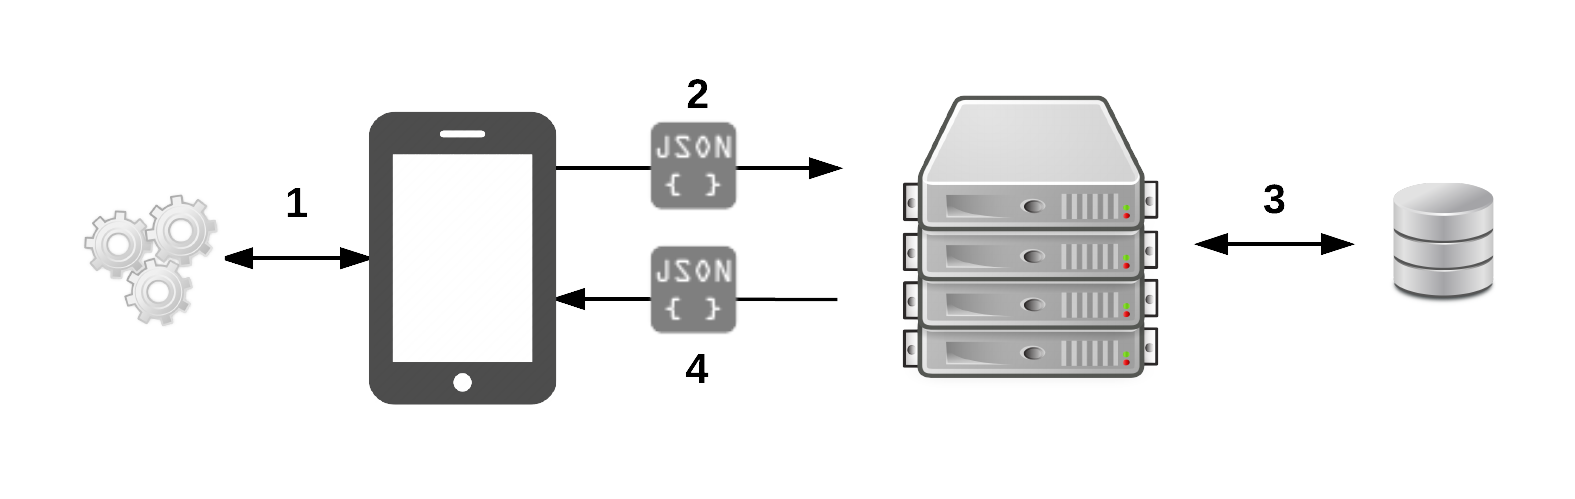
\includegraphics[scale=1]{imagenes/cap4/arquitectura_distribuida.png}
		\caption{Diagrama de la arquitectura del sistema distribuido.}
		\label{arquitectura_distribuida}
	\end{figure}

A continuación se detalla la implementación de tanto el cliente Android como el servidor y se comentan las diferencias con respecto a la versión descrita anteriormente.

\subsection{Cliente Android}
A diferencia de la versión anterior del sistema, en esta versión el cliente debe calcular los descriptores del video de consulta y realizar un petición Post al servidor enviando solo los descriptores y no el archivo de video completo. Al igual que la versión centralizada una vez obtenida la respuesta del servidor, debe mostrarle los resultados de la búsqueda al usuario. Se implementó esta versión cambiando el módulo de grabación de la cámara y el de conexión con el servidor, además se añadió un módulo de cálculo de descriptores.

\subsubsection*{Grabación}
En esta versión ya no es necesario obtener un archivo de video resultante, sino que es necesario realizar un procesamiento del video. Dada esta diferencia se decidió reimplementar este módulo, creando un nuevo fragmento \texttt{CameraPreviewFragment} de manera que se puedan obtener frames de la cámara mientras se graba el video para poder realizar el cálculo en tiempo real.

La interfaz gráfica del fragmento \texttt{CameraPreviewFragment} consta de tres elementos que podemos identificar en la figura~\ref{pantalla_camera_preview}, el preview de la cámara, los cuatro puntos con los que el usuario puede marcar los límites de la pantalla y finalmente un botón para comenzar la grabación. A continuación se detallan aspectos de la implementación de cada uno de estos elementos.

A diferencia de la versión anterior, en que la cámara era manejada por una aplicación predefinida, ahora es necesario manejar los eventos del ciclo de vida de la cámara. Para esto se utilizó la funcionalidad de la clase \texttt{Camera}\footnote{\url{http://developer.android.com/guide/topics/media/camera.html}} de Android. Esta clase permite mostrar un preview y obtener frames para procesarlos en tiempo real. Se programó la clase \texttt{CameraContainer}, que representa un elemento gráfico que contiene el preview. La clase además encapsula las llamadas al sistema operativo necesarias para controlar la cámara, a través de las funciones \texttt{startCameraPreview}, \texttt{stopCameraPreview} y \texttt{releaseCamera}.

Se programó la clase \texttt{CropView} que controla los cuatro puntos vistos en la interfaz. Estos puntos permiten al usuario ajustar el video al tamaño de su pantalla, esto permite un mejor desempeño de los descriptores utilizados dado que todo lo grabado corresponde al video de consulta y no a objetos exteriores como el marco de la pantalla. La clase contiene cuatro puntos representados por objetos de la clase \texttt{Point} e implementa el método \texttt{onTouchEvent}, que permite ser notificado por el sistema operativo cuando el usuario toca la pantalla. Cuando esto sucede se verifica si el usuario está arrastrando alguno de los puntos y se ajusta la interfaz gráfica para reflejar el cambio. Al procesar la imagen para calcular sus descriptores se especifica la posición de los cuatro puntos de manera que el cálculo solo considere la sección de la imagen que está dentro de sus límites.

Por último el bóton para iniciar la grabación corresponde a un objeto de la clase \texttt{Button} de Android, al presionar el botón se utiliza el método \texttt{setPreviewCallback} del cameraContainer para registrar un \emph{listener} que será llamado por el sistema cada vez que la cámara obtiene un nuevo frame de video, esto será usado por el siguiente módulo para realizar el cálculo de descriptores. La interfaz gráfica cambia para reflejar que se están calculando descriptores, el botón de iniciar se reemplaza por una barra de progreso que muestra cuanto tiempo de grabación queda como muestra la figura~\ref{pantalla_calculando_descriptores}.

La figura~\ref{diagrama_modulo_captura} muestra un diagrama que detalla las clases utilizadas descritas anteriormente.

	\begin{figure}[!h]
		\centering
		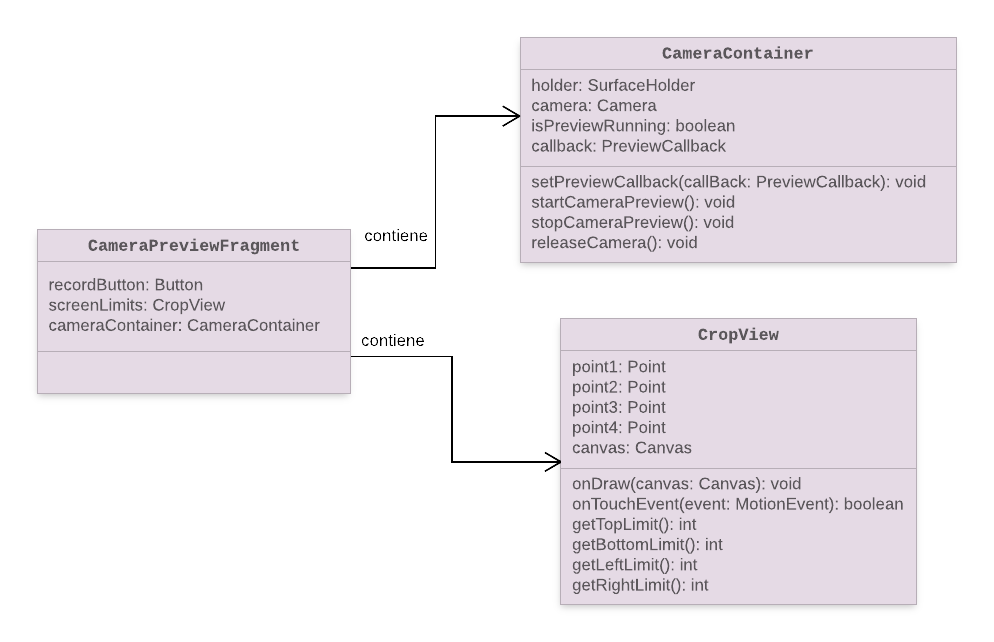
\includegraphics[scale=1.6]{imagenes/cap4/diagrama_modulo_captura.png}
		\caption{Diagrama de clases del módulo de grabación del sistema distribuido.}
		\label{diagrama_modulo_captura}
	\end{figure}

\subsubsection*{Cálculo de descriptores}
	\begin{figure}[!h]
		\centering
		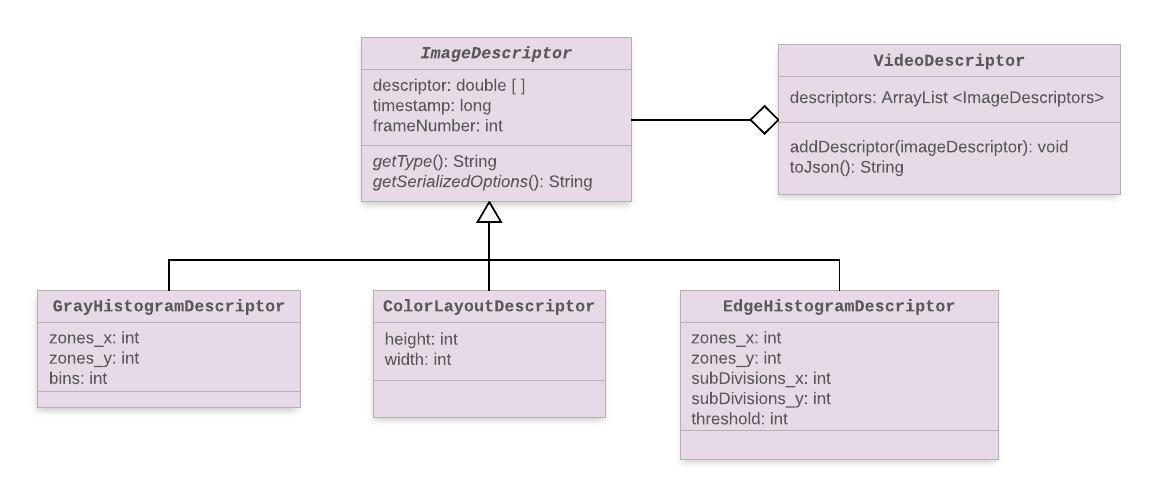
\includegraphics[scale=1.6]{imagenes/cap4/diagrama_clases_descriptores.png}
		\caption{Diagrama de las clases usadas para modelar descriptores.}
		\label{diagrama_clases_descriptores}
	\end{figure}
La figura~\ref{diagrama_clases_descriptores} muestra las clases que modelan los descriptores. Se creó la clase abstracta \texttt{ImageDescriptor} que corresponde a un descriptor de imágenes genérico, contiene un arreglo de doubles, un timestamp y un frameNumber que identifican el frame al cual corresponde el descriptor. Los métodos abstractos \texttt{getType} y \texttt{getSerializedOptions} son usados para serializar el descriptor al enviarlo al servidor. La clase tiene tres implementaciones concretas que corresponden a los tres tipos de descriptores que el sistema puede calcular.

Por otro lado está la clase \texttt{VideoDescriptor} que representa un descriptor de video, esta clase contiene una lista de descriptores de imágenes y cuenta con los métodos \texttt{addDescriptor} que recibe un descriptor de imagen y lo añade a la lista, y el método \texttt{toJson} que serializa el descriptor en formato JSON para enviarlo al servidor.


El cálculo de descriptores de imágenes es realizado por clases que implementan la interfaz \texttt{DescriptorExtractor}. Esta interfaz define el método \texttt{extract}, que recibe el arreglo de bytes con los datos de un frame de video y el timestamp y frameNumber del frame correspondiente y entrega su descriptor de imagen. La figura~\ref{diagrama_clases_extractores} muestra el diagrama de clases con las clases que implementan la interfaz. El diagrama además muestra la clase \texttt{VideoDescriptorExtractor}, esta clase se usa en conjunto con los extractores para cálcular los descriptores de un video.
	\begin{figure}[!h]
		\centering
		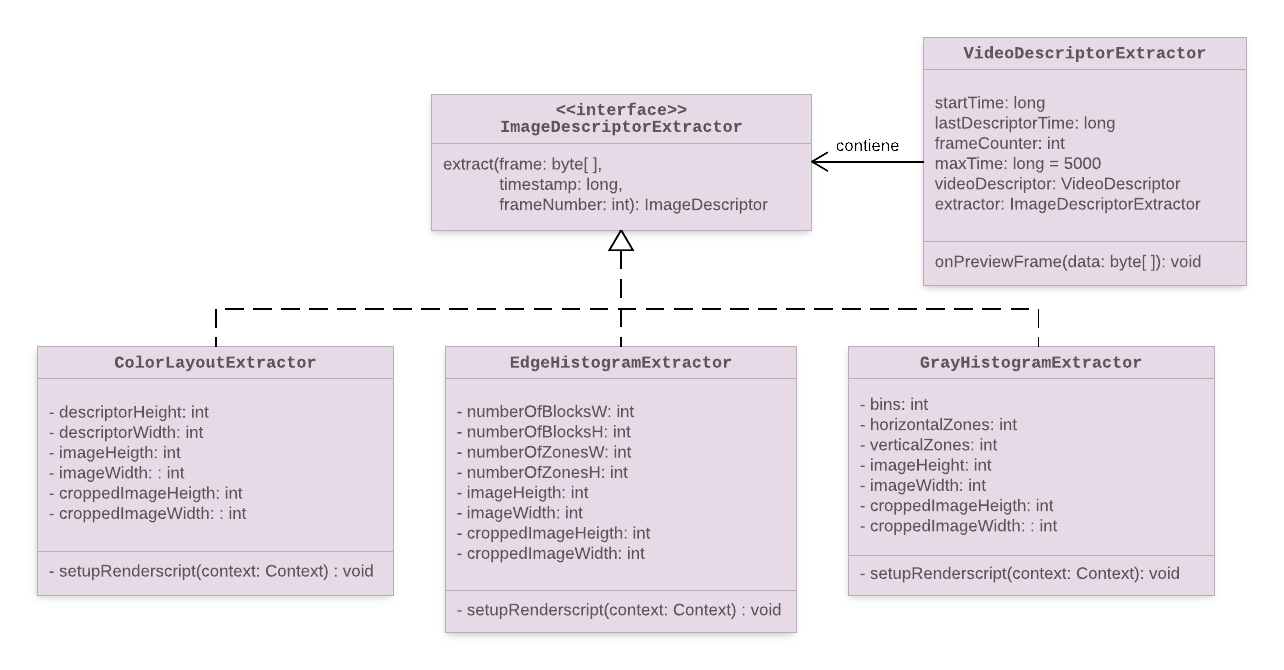
\includegraphics[scale=1.6]{imagenes/cap4/diagrama_clases_extractores.png}
		\caption{Diagrama de clases de extractores de descriptores.}
		\label{diagrama_clases_extractores}
	\end{figure}

VideoDescriptorExtractor implementa la interfaz \texttt{PreviewCallback} con lo que se puede registrar para obtener frames de la cámara. Cada frame se recibe como un arreglo de bytes en formato YUV. En este cada pixel se divide en valores de \emph{luma} (Y) que indica la intensidad de luz y \emph{chroma} (UV) que indican el color. Específicamente se usa el formato YUV420 NV21\footnote{\url{http://www.fourcc.org/yuv.php\#NV21}}, que establece un ordenamiento de los valores como indica la figura~\ref{formato_yuv}. Los primeros $W \times H$ bytes corresponden a los valores de \emph{luma} de cada pixel, donde $W$ y $H$ corresponden al ancho y alto de la imagen.  
	\begin{figure}[!h]
		\centering
		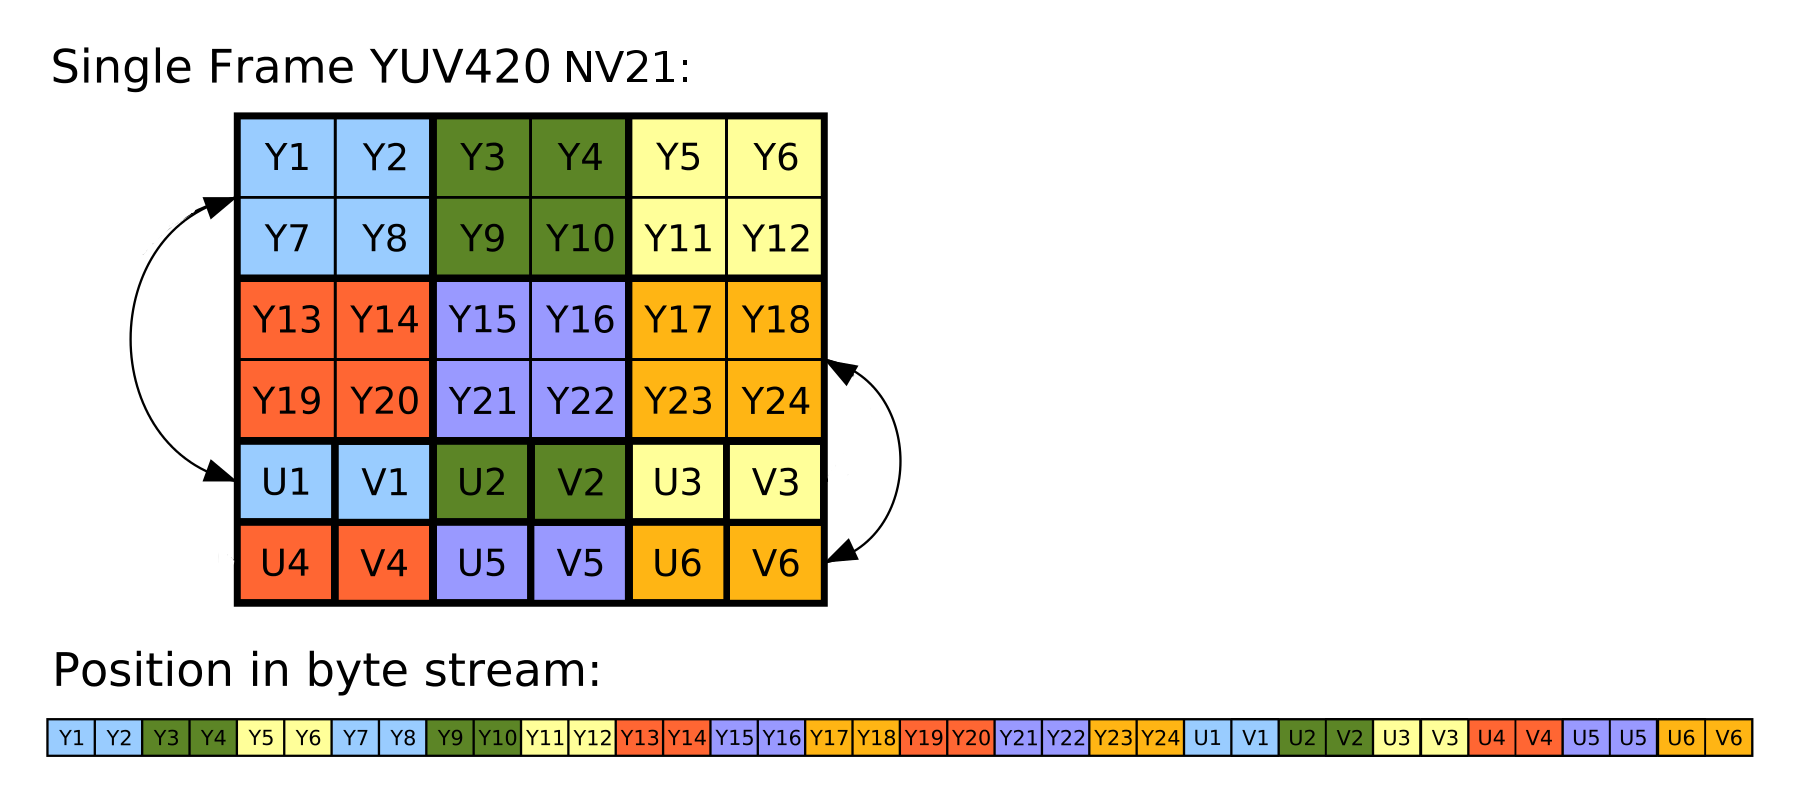
\includegraphics[scale=0.3]{imagenes/cap4/yuv.png}
		\caption{Especificación del formato YUV420 NV21.}
		\label{formato_yuv}
	\end{figure}

VideoDescriptorExtractor intenta procesar frames a un ritmo constante de 4 frames por segundo. Al recibir un nuevo frame primero verifica si se está procesando un frame anterior, de ser así se ignora el frame recibido sin procesarlo, de lo contrario se revisa el tiempo transcurrido desde el último frame procesado. Si ha pasado muy poco tiempo desde el último frame (menos de 0.25 segundos) entonces se ignora y se sigue esperando. Para procesar un frame se usa alguno de los extractores definidos en la figura~\ref{diagrama_clases_extractores}, al invocar su método \texttt{extract} se obtiene un objeto de tipo \texttt{ImageDescriptor}, este descriptor de imagen se añade a un descriptor de video mantenido por el VideoDescriptorExtractor usando el método \texttt{addDescriptor} de la clase \texttt{VideoDescriptor}.

A continuación se explica en detalle el funcionamiento de cada extractor de descriptores de imágenes implementado.

%%GRAYHISTOGRAM_EXTRACTOR
\texttt{GrayHistogramExtractor} maneja el cálculo de histogramas de grises por zona. El algoritmo para calcular el descriptor consiste de cuatro etapas:
\begin{enumerate}
\item Transformar imagen de color en formato YUV a escala de grises.
\item Croppear imagen para ajustarse a los límites establecidos por el usuario.
\item Calcular histograma, esto es, contar la cantidad de pixeles con cierta intensidad en cada zona.
\item Normalizar histograma.
\end{enumerate}

La primera etapa se logra extrayendo los primeros $W\times H$ bytes del arreglo de bytes, donde $W$ y $H$ son el ancho y alto de la imagen, en el formato YUV utilizado por Android estos corresponden a la intensidad de luz de los pixeles de la imagen, es decir, sus valores de gris. La extracción de bytes se realiza con el método \texttt{copy2DRangeFrom} de la clase \texttt{Allocation} de RenderScript, que recibe un arreglo de bytes, valores de offset horizontal y vertical, alto y ancho de la imagen y extrae los valores del arreglo para poblar una Allocation. Al final de esta etapa se obtiene una Allocation con los valores de gris de la imagen. \\

Para la segunda etapa nuevamente se usa el método \texttt{copy2DRangeFrom}, esta vez se usa una versión del método que recibe una Allocation, y valores de offset, alto y ancho para extraer un subconjunto de valores de la Allocation recibida. Al final de esta etapa se obtiene una nueva Allocation distinta a la de la etapa anterior, que contiene solo los valores de gris de la zona demarcada por el usuario.\\

La tercera etapa requiere el uso de RenderScript para realizar el cómputo. Esto se logró con el script \texttt{GrayZoneHist.rs} que itera sobre cada pixel de la imagen, calcula su bin correspondiente basado en su valor de gris y su posición y aumenta en 1 el valor del bin. Para aumentar el valor del bin se debe usar una primitiva de sincronización, de lo contrario podrían ocurrir \emph{data races} dado que el script se ejecuta en parlelo. Se utilizó la función \texttt{rsAtomicInc} que recibe una dirección de memoria e incrementa su valor en 1 de forma atómica. La allocation de salida del script contiene el histograma sin normalizar. El código del script \texttt{GrayZoneHist.rs} se encuentra adjunto en la sección de Anexos.

En la cuarta etapa primero se extrae el contenido de la Allocation que contiene el histograma y se copia a un arreglo de ints. Esto se logra con el método \texttt{copyTo} de la clase \texttt{Allocation}. Luego se crea un nuevo arreglo de doubles que contendrá el histograma normalizado. Se itera sobre el histograma dividiendo cada valor por la cantidad de pixeles en su zona correspondiente y asignando el resultado al histograma normalizado. Finalmente se crea un objeto \texttt{GaryHistogramDescriptor} con el histograma normalizado y se retorna.

%%KEYFRAME_EXTRACTOR
\texttt{KeyframeExtractor} maneja el cálculo del descriptor reduced keyframe. El algoritmo para calcularlo toma los siguientes pasos:
\begin{enumerate}
\item Transformar imagen de formato YUV a formato RGB.
\item Croppear imagen para ajustarse a los límites establecidos por el usuario.
\item Calcular el promedio de color por canal en cada zona.
\end{enumerate}

El primer paso se logra usando la clase \texttt{ScriptIntrinsicYuvToRGB} de RenderScript. Esta clase pertenece a la biblioteca de RenderScript y permite decodificar una imagen en YUV y pasarla a formato RGB, solo es necesario crear Allocations de entrada y salida del tamaño correspondiente. El resultado es una Allocation que contiene la imagen en formato RGB.

El segundo paso se logra de la misma manera que en el extractor anterior, usando el método \texttt{copy2DRangeFrom} de la clase Allocation. El resultado de este paso es un Allocation que contiene los valore RGB de la sección de la imagen indicada por el usuario.

El tercer paso se realiza usando RenderScript con el script \texttt{keyframe.rs}. Este script itera sobre cada pixel de la imagen y separa el pixel en sus valores de rojo, verde y azul. Cada valor es sumado a un contador correspondiente a su zona. Para realizar esta suma se usó la función \texttt{rsAtomicAdd} de RenderScript que permite realizar sumas de manera atómica. La Allocation de salida contiene la suma de los valores de rojo, verde y azul de los pixeles de cada zona. Para calcular el valor promedio de cada color basta dividir el valor obtenido por el script por la cantidad de pixeles de cada zona. Para esto se extrae el contenido de la Allocation usando el método \texttt{copyTo} al igual que en el extractor anterior. Luego se itera por cada valor y se divide por la cantidad de pixeles de la zona. Finalmente se crea un objeto \texttt{KeyframeDescriptor} y se retorna. El código del script \texttt{keyframe.rs} se encuentra adjunto en la sección de Anexos.
 
%%EDGEHISTOGRAM_EXTRACTOR
La clase \texttt{EdgeHistogramExtractor} se encarga del cálculo del descriptor de histograma de bordes. Los pasos del algoritmo para el computo son los siguientes:
\begin{enumerate}
\item Transformar imagen de color en formato YUV a escala de grises.
\item Croppear imagen para ajustarse a los límites establecidos por el usuario.
\item Reducir la imagen a una cantidad fija de bloques, donde el valor de cada zona corresponde al promedio del valor de los pixeles dentro de la zona.
\item Calcular la energía de cada filtro aplicándolo sobre grupos de cuatro bloques. Se selecciona el mayor y se revisa si la energía correspondiente excede un valor umbral.
\item Calcular el histograma de bordes, que indica por zona cuantos grupos de bloques presentan cada uno de los tipos de bordes posibles.
\item Normalizar el histograma.
\end{enumerate}

Las primeras dos etapa son idénticas a las primeras etapas del cálculo del descriptor de histograma de grises y se realizan de la misma forma. El resultado al final de la segunda etapa es un Allocation con los valores de gris correspondiente a la sección de la imagen seleccionada por el usuario.

La tercer etapa es similar al cálculo del descriptor reduced keyframe y se realiza de forma análoga. El script \texttt{reducer.rs} divide la imagen en bloques e itera sobre cada pixel sumando su valor de gris al de la zona correspondiente. El resultado del script es una Allocation con la suma de los pixeles en cada zona. Al igual que en el descriptor anterior se extraen los resultados a un arreglo usando el método \texttt{copyTo} y se divide cada valor por la cantidad de pixeles por zona, con esto se obtiene un arreglo con el valor de gris promedio en cada zona.

Para la cuarta etapa se toma el arreglo resultante del paso anterior y se usa para poblar una Allocation. Estos datos se usan como entrada para el script \texttt{borderDetector.rs}, que toma grupos de cuatro bloques y calcula el valor de energía de cada filtro, selecciona el mayor y se prueba si pasa el valor umbral. La Allocation de salida contiene un número del 0 al 5 por cada bloque, si el filtro de mayor energía pasó el valor umbral, el valor irá de 0 a 4 indicando el indice del filtro de mayor energía, en caso que el mayor no supere el umbral se marcará con un 5.

La quinta etapa es similar al cálculo de histograma de grises. El script \texttt{edgeHist.rs} itera sobre cada bloque revisando cual fue el filtro de mayor energía, para cada zona se cuenta la cantidad de bloques con cada tipo de borde. Si para algún bloque el valor en la Allocation de entrada es 5 (correspondiente a los bloques en que la energía no excedió el umbral) no se considera para la construcción del histograma. La Allocation de salida contiene el histograma con la cantidad de bloques con cada tipo de borde por cada zona de la imagen.

La última etapa es idéntica a la última etapa de la construcción del descriptor de histograma de grises. Se extraen los valores de la última Allocation a un arreglo y se normaliza dividiendo cada valor por la cantidad de pixeles presentes en cada zona. El arreglo resultante contiene el histograma normalizado, que se usa para construir un objeto \texttt{EdgeHistogramDescriptor} y retornarlo.

Todos los script usados por EdgeHistogramExtractor se adjuntaron en la sección de anexos.\\

El proceso de cálculo de descriptores se realiza por un tiempo determinado por el VideoDescriptorExtractor. Una vez terminado el proceso se procede a enviar el descriptor de video resultante al servidor para realizar una consulta.

\subsubsection*{Conexión con el servidor}
 El módulo de conexión con el servidor es análogo al de la versión anterior. Se implementó la clase \texttt{FromDescriptorsVideoSearch} que maneja el envío de datos al servidor. A diferencia de la versión anterior esta clase recibe un objeto de la clase \texttt{VideoDescriptor} para reapizar la búsqueda. El descriptor de video puede ser serializado con su método \texttt{toJson}, este método usa los métodos \texttt{getType} y \texttt{getSerializedOptions} de los descriptores de imágenes para obtener propiedades del descriptor necesarias para la búsqueda como el tipo de descriptor y su tamaño. Una vez serializado se envía al servidor usando la clase \texttt{HttpUrlConnection} de Java. Al igual que la versión anterior una vez se termina de enviar datos al servidor se cambia la interfaz gráfica de la aplicación, a una pantalla inicialmente vacía donde se mostrarán los resultados.

\subsubsection*{Interfaz de resultados}
Este módulo no presenta diferencias con respecto a la versión anterior, se reutilizó la clase \texttt{QueryResultsFragment} para mostrar los resultados obtenidos del servidor.\\

La figura~\ref{diagrama_cliente_distribuido} muestra un diagrama de clases resumido con las clases que componen la versión distribuida del cliente.
	\begin{figure}[!h]
		\centering
		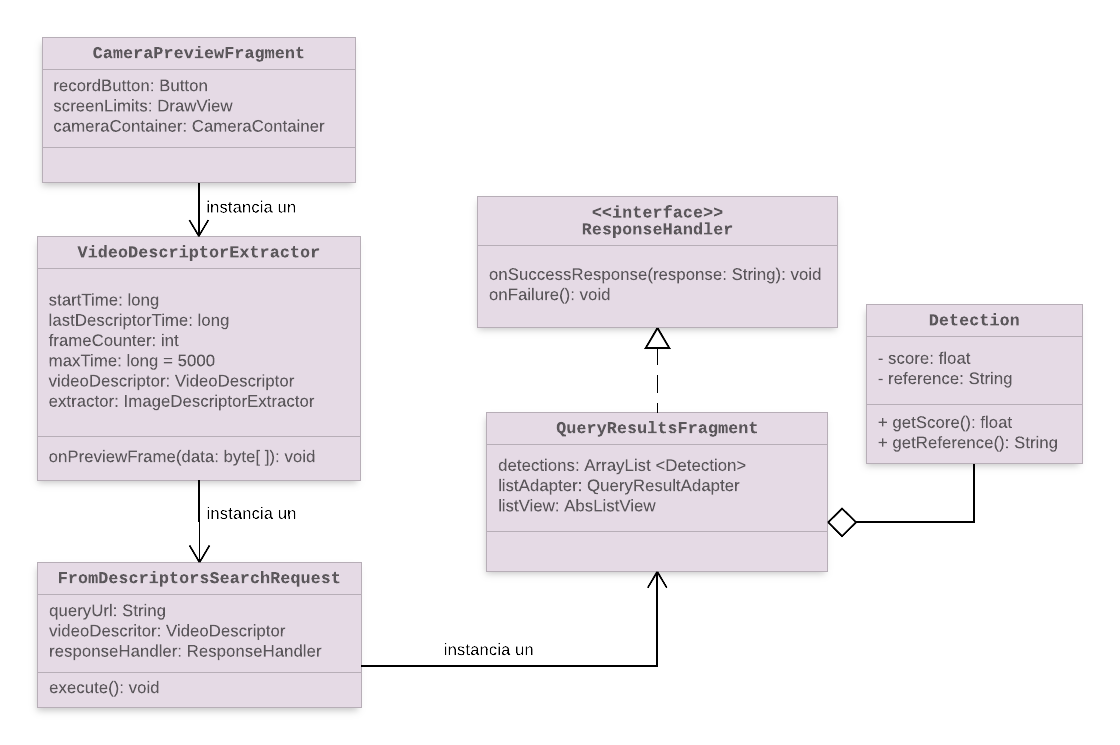
\includegraphics[scale=1.6]{imagenes/cap4/diagrama_cliente_distribuido.png}
		\caption{Diagrama de clases del cliente distribuido.}
		\label{diagrama_cliente_distribuido}
	\end{figure}

\subsection{Servidor}

La implementación de la versión distribuida del servidor es análoga a la versión centralizada. Se creó la función \texttt{search\_by\_descriptors} que sirve la URL usada por el cliente para enviar los descriptores. Se reutilizaron las funciones \texttt{new\_search\_profile}, \texttt{search} y \texttt{detect} del módulo \texttt{PVCD\_Wrapper}. 

Dado que esta versión recibe los descriptores en vez del video completo basta con guardar los descriptores con el formato apropiado para realizar la búsqueda. Además de esto es necesario crear los archivos que identifican la base de datos del video de búsqueda, ya que a pesar que el video no está en el servidor (ni se utiliza en ningún paso de la búsqueda) P-VCD exige que exista una base de datos con su correspondiente segmentación. Se crearon funciones que imitan el funcionamiento de P-VCD, creando una base de datos, una segmentación y un archivo de descriptores a partir de la información recibida por el servidos. A continuación se describen las nuevas funciones implementadas.

\begin{itemize}

\item{\texttt{create\_database}} 

Esta función crea una base de datos vacía. Crea una carpeta con un archivo \texttt{files.txt}, normalmente este archivo contiene información del video, como la ruta a su archivo, tipo de archivo, etc. Esta información es usada por P-VCD para extraer la segmentación y los descriptores. Dado que estas operaciones no son necesarias en esta versión del sistema se puede crear el archivo \texttt{files.txt} con los headers apropiados pero con sin información. 

\item{\texttt{create\_segmentation}} 

Al crear una segmentación P-VCD extrae información de cuales frames serán usados por el sistema para calcular descriptores. Se especifica el número del frame correspondiente y el instante en que este aparece en el video. Toda la información necesaria para crear la 
segmentación es enviada al servidor junto con los descriptores del video. El cliente envía una lista con los números de frame y el instante en que aparecieron, la función usa esta información para crear el archivo \texttt{query.seg} requerido por el sistema. 

\item{\texttt{write\_descriptors}} 

Los descriptores requieren dos archivos, uno con información sobre el tipo de descriptor y sus parámetros, y otro con los valores del descriptor mismo. La función crea ambos archivos, el primero, \texttt{descriptor.des}, se escribe con la información recibida desde el cliente con las opciones del descriptor. El archivo \texttt{query.bin} corresponde al contenido de los descriptores, este se escribe usando la clase \texttt{array}\footnote{\url{https://docs.python.org/2/library/array.html}} de Python, esta clase permite escribir un arreglo numérico en un archivo binario con la función \texttt{to\_file}.  
\end{itemize}

La función \texttt{search\_by\_descriptors} ejecuta las tres nuevas funciones para crear los archivos necesarios para la búsqueda. Después de esto la búsqueda procede idénticamente a la versión anterior.

Esta versión del sistema soluciona los problemas expuestos en la sección anterior. Al enviar solo los descriptores de video al servidor se disminuye significativamente el uso de la red de datos, lo cual además reduce el tiempo de respuesta del sistema. Por otro lado se disminuye la carga del servidor al realizar la extracción de descriptores en el dispositivo móvil.

En el siguiente capítulo se exponen las pruebas realizadas con el sistema, que buscan determinar empíricamente las diferencias entre ambas versiones del sistema en términos de tiempo de respuesta y uso de recursos del sistema. Además se busca comparar la eficacia de los descriptores usados para realizar la búsqueda. 